% !TeX root = ../main.tex
% Add the above to each chapter to make compiling the PDF easier in some editors.

\chapter{Integration into existing App}\label{chapter:Integration into existing App}

\section{Overview and existing functions of App}
The App I had to build upon, already had some features related to the open source car driving simulator "Speed Dreams", but before we go deeper into theses functionalities, I am going to start with the present structure and Appearance.
First of all, a dark theme has been chosen for the design of the App. As can be seen in Figure \ref{fig:main_screen}, the main screen contains different tiles for each task. It is possible to choose the source of intended input, therefore the user decides between loading an existing image (Figure \ref{fig:load_image}), or hitting the camera icon to call a life-video feed of the back-facing camera. Depending on which input source has been chosen, the functionalities are applied either one single time or multiple times per second, both ways the outputs are printed onto the original images. Both features, that are named "Vehicle Detection" and "Lane Detection" are pretty much self explaining, but it should be mentioned that both methods are very likely trained by "Speed Dreams" data, meaning that the Lane detection is good for detecting lanes in the game, but might not be that brilliant in detecting real lanes, furthermore the vehicle detection recognizes only the back of the red car in the virtual rally course. 


\begin{figure}[H]
	\minipage{0.33\textwidth}
	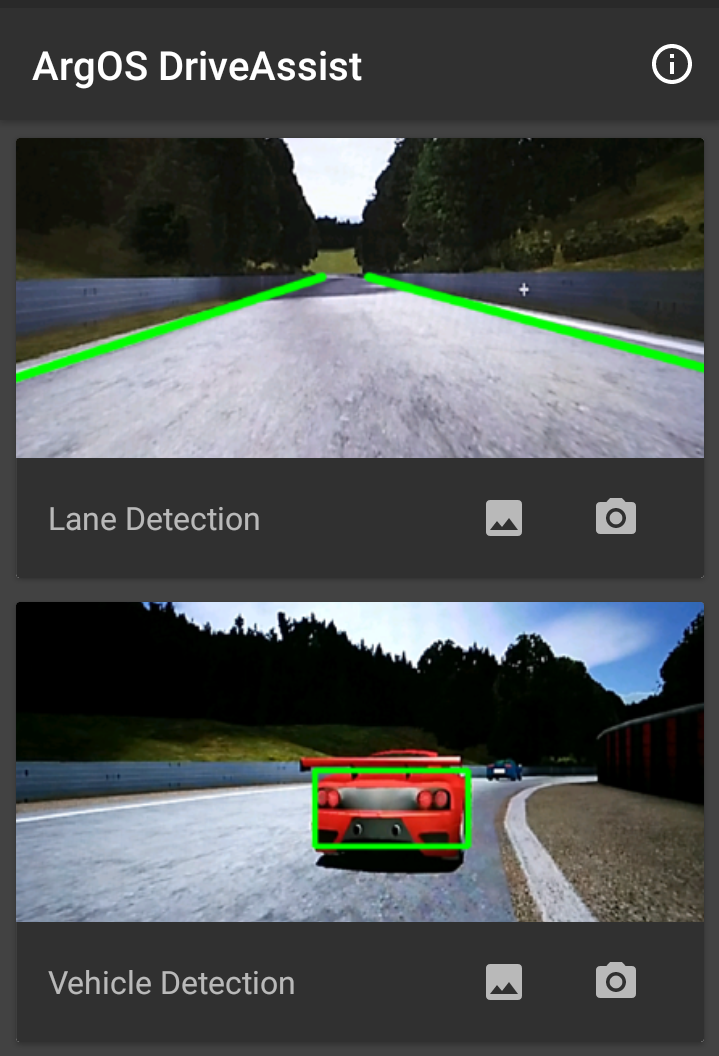
\includegraphics[width=\linewidth]{images/screenshot_main.png}
	\caption{Main screen}\label{fig:main_screen}
	\endminipage\hfill
	\minipage{0.33\textwidth}%
	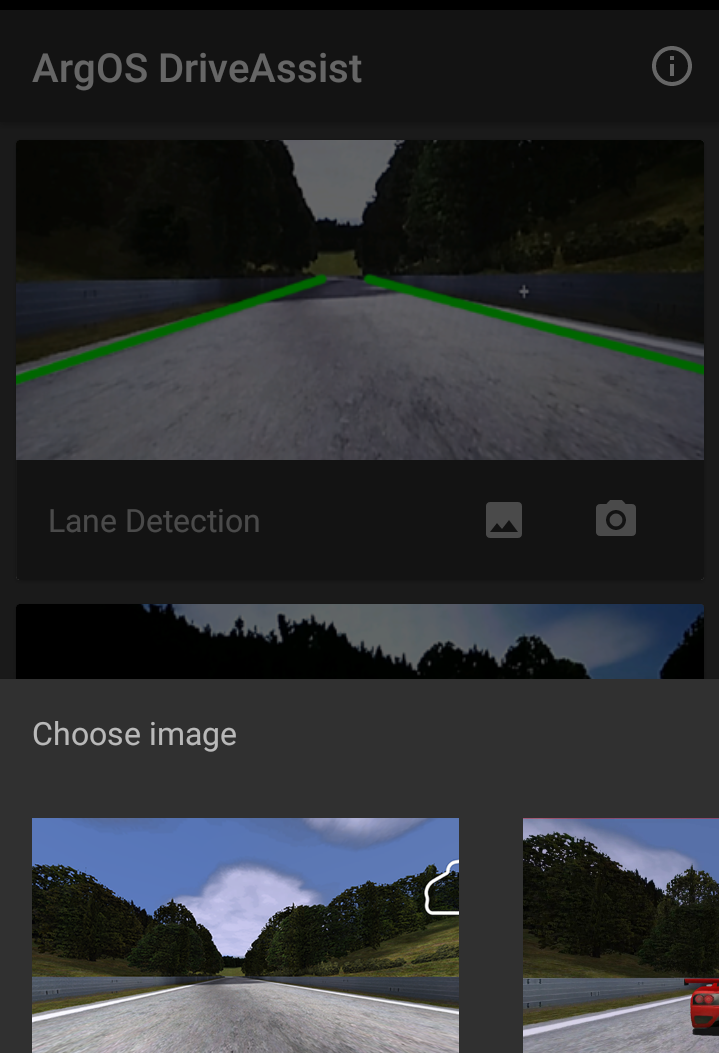
\includegraphics[width=\linewidth]{images/screenshot_load_image.png}
	\caption{Load Image}\label{fig:load_image}
	\endminipage\hfill
	\minipage{0.33\textwidth}
	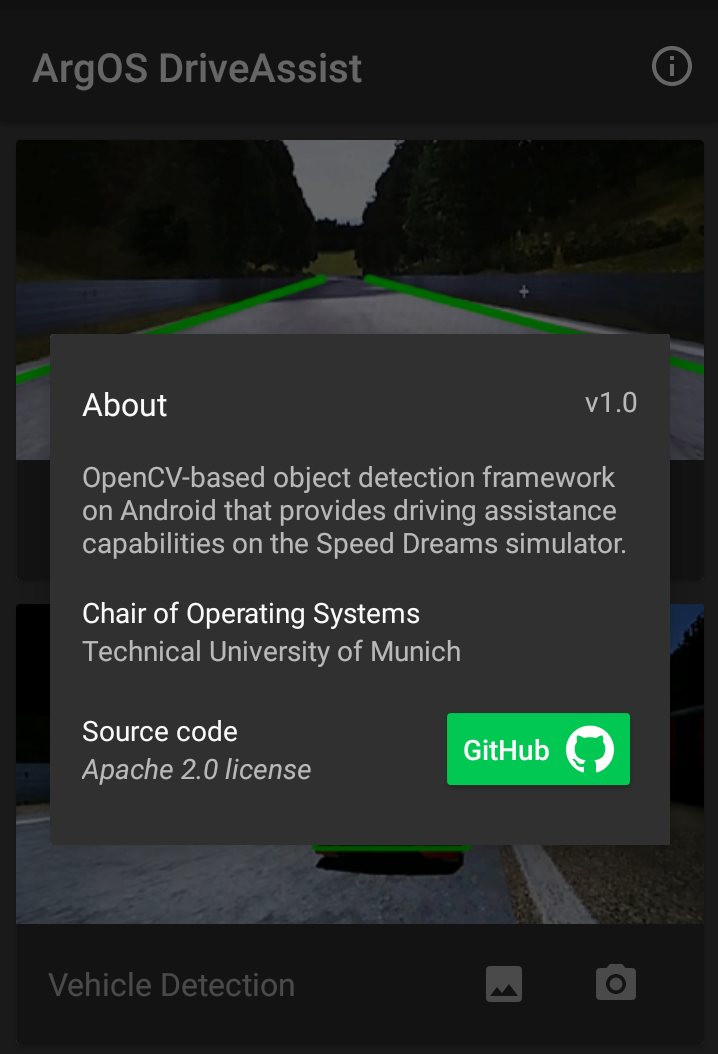
\includegraphics[width=\linewidth]{images/screenshot_about.png}
	\caption{About}\label{fig:about}
	\endminipage

\end{figure}


